% =====================================================================
%  rtt_shock.tex -- the manual's figure of chapter 3 (Shock waves). Drawn
%  from the ME 697 Unit 3 sheet's figure (Equation_Sheets/Unit_03_rev-1/rtt_shock.tex,
%  D. E. Kittell), which stays the sheet's; this copy is the manual's.
%  Built by 'make manual'.
% =====================================================================
\documentclass[tikz,border=10pt]{standalone}
\usetikzlibrary{arrows.meta}

% ---- Muted academic theme ----
\definecolor{slate}{HTML}{2C3E50}
\definecolor{oiblue}{HTML}{0072B2}
\definecolor{oiorange}{HTML}{E69F00}
\definecolor{oigreen}{HTML}{009E73}
\definecolor{oivermil}{HTML}{D55E00}

\tikzset{
  axis/.style = {-{Stealth[length=6pt]}, slate, thin},
  data/.style = {oiblue, very thick},
  qdata/.style= {oiorange, line width=1.2pt},
  cv/.style   = {slate, thick, densely dashed},
  flow/.style = {-{Stealth[length=8pt, width=6pt]}, oigreen,
                 line width=1.4pt},
}

\begin{document}
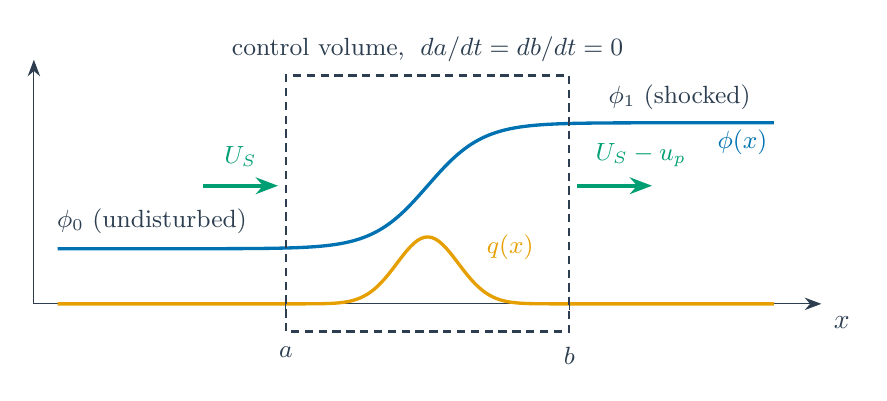
\begin{tikzpicture}[font=\sffamily, text=slate]
  \def\xc{5.0}    % front center
  \def\a{3.2}     % CV left boundary
  \def\b{6.8}     % CV right boundary

  % axes
  \draw[axis] (0,0) -- (10.0,0) node[below right=1pt] {$x$};
  \draw[axis] (0,0) -- (0,3.1);

  % phi(x): tanh shock profile (undisturbed left -> shocked right)
  \draw[data] plot[domain=0.3:9.4, samples=200]
      ({\x}, {1.5 + 0.8*tanh((\x-\xc)/0.7)});
  \node[font=\small] at (1.5, 1.05) {$\phi_0$ (undisturbed)};
  \node[font=\small] at (8.2, 2.62) {$\phi_1$ (shocked)};
  \node[font=\small, text=oiblue] at (9.0, 2.05) {$\phi(x)$};

  % q(x): nonzero only inside the front
  \draw[qdata] plot[domain=0.3:9.4, samples=200]
      ({\x}, {0.85*exp(-((\x-\xc)/0.55)^2)});
  \node[font=\small, text=oiorange] at (6.05, 0.72) {$q(x)$};

  % flux arrows (shock frame; material flows left -> right)
  \draw[flow] (2.15, 1.5) -- (3.1, 1.5)
      node[midway, above=3pt, text=oigreen, font=\small] {$U_S$};
  \draw[flow] (\b+0.1, 1.5) -- (7.85, 1.5)
      node[pos=0.85, above=3pt, text=oigreen, font=\small] {$U_S-u_p$};

  % x ticks at a, b
  \foreach \xx/\l in {\a/$a$, \b/$b$} {
    \draw[slate, thin] (\xx, -0.08) -- (\xx, 0.08);
    \node[below=2pt, font=\small] at (\xx, -0.35) {\l};
  }

  % control volume (dashed, drawn last)
  \draw[cv] (\a, -0.35) rectangle (\b, 2.9);
  \node[above, font=\small, align=center] at (\xc, 2.95)
      {control volume,\; $da/dt = db/dt = 0$};
\end{tikzpicture}
\end{document}
